\chapter{Technical foundations}
\label{cha:technicalfoundations}

Before any explanation of the theoretical approach behind this research, there is a need of describing the technical foundations, on which the general thoughts were built on.

Being mostly a back-end web developer since the start of my studies, I experienced a lot of changes in this field. Changes which were mostly caused by the ongoing progression of general web development, but also caused by constantly coming and going ``hypes''. Changes which mostly left minor traces, but sometimes had a major impact on the way I process things during my work on different projects.

\paragraph{} % EcmaScript 6.
One of these major turning points was the introduction of EcmaScript 6 (\texttt{ES6}), which I first heard from in a talk given by \emph{Douglas Crockford}\footnote{\url{http://crockford.com} -- Douglas Crockford's website.} in March 2015. He is -- besides other projects -- not only the creator of \texttt{JSLint} \cite{JSLintDocumentation}, but also the author of ``\emph{The Good Parts}'' \cite{crockford2008javascript}, a language reference for \texttt{JavaScript}.

\texttt{ES6} introduced a lot of new features, pushing \texttt{JavaScript} more and more towards the definition of an ``object-oriented'' scripting language, thus not only by providing ``real classes'', instead of the old and cumbersome approach of inheritence by setting a constructor function into the \texttt{prototype} object \cite[47]{crockford2008javascript}.

However, the probably most beneficial functions are \texttt{Promises} \cite{MDNPromise} and \texttt{Arrow functions} \cite{MDNArrowFunctions}, both saving significant amounts of code -- especially when working with asynchronous environments, like HTTP requests.

\paragraph{} % Static site generation.
Ever since I first got to work with a static site generator, I got more and more interested in how easy and fast static site projects may be scaffolded. Once completely set up, I was simply impressed by its power and variety -- this differed completely from the dynamic web environments I used to work with at that time.

A dynamic web project often demands lots of preparation before receiving any visible outcome, sometimes even when using a predefined framework. Additionally, though many projects in the \texttt{Node.js} universe are already matured to an extent, where they may be even used for enterprise projects, there is still a remaining risk for failing a client due to the amount of dependencies on external services like databases, session storages or user management tools.

\section{Build pipelines}
\label{sec:buildpipelines}

%% Graphic of build pipeline components
\begin{figure} % h-ere, t-op, b-ottom, p-age
    \centering
    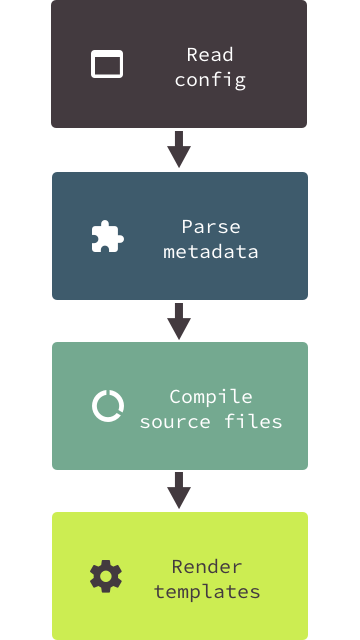
\includegraphics[width=0.9\textwidth]{build_pipeline.png}
    \caption{A graphic showing the basic flow of a \emph{build pipeline}.\\
    First, the configuration file is read and necessary modules invoked. Second, the global metadata, as well as metadata from within the content, is parsed and stored in the global configuration. Third, the content sources get compiled into basic \emph{HTML} markup. Last, the compiled content gets rendered into predefined templates, to apply a given structure which is used commonly throughout the website.}
    \label{fig:build-pipeline}
\end{figure}
%

A static site generator mostly consists of a build pipeline, which handles the workflow needed for bringing the content into shape. This goes from setting the boundaries, determined by a configuration file, to finally producing a web root, consisting of HTML, CSS and JavaScript files, as well as images.

Normally, the major part of it happens sequentially, as nearly all content files are facing a series of transformations on them \cite{Metalsmith2015technicaldocumentation}. Although the amount and extent of conversions may differ significantly from pipeline setup to pipeline setup, it can be broken down to the following core parts (see Fig. \ref{fig:build-pipeline}):

\begin{description}
  \item[Metadata parser] -- Parses global metadata, found in the configuration file or in the YAML frontmatter of content files.
  \item[Markdown compiler] -- Used to convert easily read- and writeable Markdown files in browser-readable HTML.
  \item[Template renderer] -- Responsible for bringing the very basic content structure in shape. The goal should be a common appearence, enriched with additional elements (like navigation, breadcrumbs, \ldots).
\end{description}

Of course, the list above overlaps at some point with the list mentioned in <<\emph{\nameref{par:creatingcontent}}>> on p. \pageref{par:creatingcontent}, as I consider a build pipeline just as a part of the given static site generator (although the main part), not as the generator itself. One of the reasons is its independence of programming languages: A build pipeline doesn't care which programming language it consists of, as long as it knows how to interpret the content sources and templates. Therefore, I may call it merely a concept, not a framework.

%% Say something about the config file, yadda yadda yadda one hand pure build pipeline, because of metadata and configuration, other hand no, because of plugins. plugins??

\subsection{Frontmatter}
\label{sec:buildpipelines-frontmatter}

\lstinputlisting[caption={frontmatter.md}, label={list:frontmatter}]{chapters/03-technical-foundations/_support/frontmatter.md}

listing \ref{list:frontmatter} shows a sample usage of frontmatter inside a Markdown file. Bounded by three dashes above the main content source, it allows certain per-file metadata definitions, which will be parsed at build time and provided for the template rendering engine.
% Mention something about omitting databases using frontmatter meta

As an example, the selected template for this sample file may also hold a list for the mentioned \emph{tags}, as well as a placeholder for the \emph{author}'s name and/or \emph{title}. The main content gets then rendered into the respective placeholding tag, already self-containing a basic structure.

Using a \emph{template: false} declaration, some plugins may prevent rendering the content into a template. This might be interesting in cases, where different partials should be included in the DOM by some sort of asynchronous JavaScript later on.


% TODO: Ugly, remove if not necessary anymore, cares for vertical spaces above subsections
\vspace{20pt}

\subsection{Markdown}
\label{sec:buildpipelines-markdown}

\lstinputlisting[caption={markdown.md}, label={list:markdown-demo}]{chapters/03-technical-foundations/_support/markdown.md}

\texttt{Markdown} consists of shorthand conventions, which should be easier to type for content creators  \cite[38]{dhillon2016}.
Therefore, it makes understanding \texttt{HTML} not a necessary precondition anymore, as a basic content structure may be easily achieved when prepending/surrounding text with certain special characters like \texttt{\#, *, \_, \ldots} (See Listing \ref{list:markdown-demo}).

Originally created by \emph{John Gruber}\footnote{\url{http://daringfireball.net/projects/markdown/} -- Markdown website.} as a plugin for \emph{Movable Type} and \emph{Blosxom} blogging engines \cite{Markdown2004introduction} in March 2004, it should be a supportive tool for users against the complexity of formal markup languages (e.g. \texttt{HTML5}) \cite[4]{RFC7764}. According to \emph{Gruber's} intention, there is no ``invalid'' \texttt{Markdown}, as he suggests the author should either ``keep on experimenting'' or ``change the processor'', if the output happens to fail his/her expectations \cite[5]{RFC7764}.

\texttt{GitHub} finally adapted \texttt{Markdown} to its own version, called ``GitHub Flavored Markdown'' (\emph{GFM}). The people behind it enhanced its original functions to also support \emph{code blocks, tables, strike-through text}, as well as \emph{auto-linking} URL structures in the content \cite[18]{RFC7764}. Additionally, also \texttt{GitHub}-specific functions, such as \emph{user mentions, commit references} or \emph{emojis}, may be used\footnote{\url{https://guides.github.com/features/mastering-markdown/\#GitHub-flavored-markdown} -- GitHub Flavored Markdown cheat sheet on \texttt{GitHub}.}.

Since then, \texttt{GitHub} renders browser-friendly versions of general descriptions written in \texttt{Markdown}, for providing fast and easy overviews of the respective repository. As an example, an existing \texttt{README.md} always appears below the root file tree section on a repository front page \cite[5]{gandrud2013github}.


% TODO: Ugly, remove if not necessary anymore, cares for vertical spaces above subsections
\vspace{20pt}

\subsection{Templates}
\label{sec:buildpipelines-templates}

\emph{Templates} are the frames of each content page, caring for a common, browser-readable HTML structure. A uniform design layout allows site-wide look and feel using a global CSS style sheet, as well as certain events triggered by user behaviour, handled by a single JavaScript file.

Born out of the need to fail-safe produce HTML on the server, as the produced data chunks -- initiated by a client HTTP request -- steadily grew, the goal behind templating engines is primarily to separate business logic from data display. Ideally, at the end of the day, there should be no code in HTML, and no HTML in code \cite[225]{Parr2004templates}.

\begin{program}
  \caption{post.hbs}
  \label{list:handlebars}
\lstinputlisting[language=HTML]{chapters/03-technical-foundations/_support/post.html}
\end{program}

A simple template file example for a blog post is shown in Program \ref{list:handlebars}. It is written in \emph{Handlebars}, a very basic templating language, offering only a very limited amount of template logic. Included are \emph{loops, if/else, partials,~\ldots}~--~however, additional ``\emph{helper}''-functions may be added by the developer.

Although such template logic may come in handy for the most part, as some business logic decisions seem to be rather taken during rendering, instead of being hard-coded before, the concept of data separation is therefore often unknowingly violated \cite[228]{Parr2004templates}. Thus, the choice of the ``optimal'' templating engine for a given project is crucial, as different engines offer a different range of built-in logic. This could go from very conservative \emph{Mustache}\footnote{\url{https://mustache.github.io/} -- Mustache website.} to very powerful ones like \emph{Liquid}\footnote{\url{https://help.shopify.com/themes/liquid} -- Shopify's Liquid template engine.} (see Sec. \ref{sec:jekyll-technology}) or \texttt{EJS}\footnote{\url{http://www.embeddedjs.com/} -- Embedded JavaScript website}.


\section{Git}
\label{sec:git}

Today, hardly any software project is started without any form of version control system (\texttt{VCS}). It supports developers as a back-up system and living archive of their work, as data generally is ephemeral and can be lost easily \cite[1]{loeliger2012version}. Although there are many different variations offered, some of the most popular today are \emph{Git, Apache Subversion, Mercurial} and \emph{Bazaar}.

\subsection{History}
\label{sec:git-history}
\texttt{Git} was initially published by \emph{Linus Torvalds} on April 7\textsuperscript{th}, 2005 \cite[6]{loeliger2012version}. This was necessary, as the ``free'' version of the then used VCS for the \emph{Linux} kernel development, \texttt{BitKeeper}, was restricted in a way it was not suitable any longer for the community behind it. Furthermore, the search of an already available alternative to the \texttt{BitKeeper} system failed due to an unsatisfying combination of needed features, so \emph{Torvalds} came up with his own VCS flavor, containing all desired functionalities for further \emph{Linux} development (among others) \cite[4]{loeliger2012version}:

\begin{itemize}
  \item Distributed development
  \item Handle thousands of developers
  \item Efficient performance
  \item Support branched development
  \item Free, as in freedom
\end{itemize}

While it was merely a tool for kernel hackers in the beginning, its simplicity quickly made developers use it for other projects too. However, the CLI still scared off people with less programming background, until \texttt{GitHub} came and introduced its Desktop client\footnote{\url{https://desktop.github.com/} -- GitHub Desktop client.}. Today, it is one of many GUIs, which are available for different operating systems\footnote{\url{https://git-scm.com/downloads/guis} -- Git GUI clients on the \texttt{Git} website.} and completely omits the necessity of terminal emulator knowledge when working with \texttt{Git}.

%% Write something, why it is so famous. distributed development - other use cases .. blargh.

\subsection{Technology}
\label{sec:git-technology}
Having decided to use \texttt{Git} as VCS, everything begins with setting up a new respository. This can be made remotely on a service like \texttt{GitHub}, or locally using \texttt{git init}. When initialized a local repository, it can still be published remotely through setting the correct URL using \texttt{git remote} later on \cite[198]{loeliger2012version}.

\subsubsection{Commits}
The next step would be working with the repository. For the most part, this should not influence the developer's workflow in any way, as the \texttt{.git} directory should be automatically hidden in most modern editors to not distract him/herself from the actual work. If the developer succeeded in a sub-task or simply wanted to save the current project state, he/she would create a \emph{commit}.

A \emph{commit} is a snapshot of the current repository's state. While it does not contain a copy of every file and directory in the project tree, it rather compares the current condition with its predecessing snapshot and creates a list of affected files and their changes. Blobs\footnote{\emph{BLOB} -- Binary Large OBject, a file which does not consist of queryable source code.} are either reused, if they remain unchanged or created new, if they were altered\cite[65]{loeliger2012version}.

Every \emph{commit} is organized in a way, that it is chained to its predecessor (\emph{parent}), thus representing a singly linked list with the ability of gaplessly going back from the current state (\emph{head}) to the initial \emph{commit} \cite[204]{dhillon2016}\cite[65]{loeliger2012version}. This is necessary, as it may happen to fix a bug or improve a design decision only by reworking a certain snapshot in the past \cite[151]{loeliger2012version}.

\subsubsection{Branches}

%% Graphic of git branches
\begin{figure} % h-ere, t-op, b-ottom, p-age
    \centering
    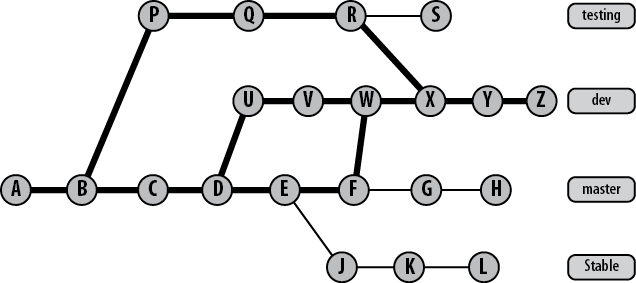
\includegraphics[width=0.8\textwidth]{git-branches.png}
    \caption{A graphic showing the basic structure of branches in \texttt{Git}.\\
    The \textbf{testing} branch was created out of project state ``B'', whereas \textbf{dev} was branched away from state ``D'' and currently holds the \emph{head commit} at ``Z''. In the meantime, \textbf{testing} was merged into \textbf{dev} at state ``R''. In the end, \textbf{dev} contains the commit history of all states connected with the bold line \cite[p. 92f]{loeliger2012version}.}
    \label{fig:git-branches}
\end{figure}
%

Since its early days, \texttt{Git} was used not only as back-up or archive system, but also as code management system. This is possible due to built-in functions, such as the so-called \emph{branched development}, where a current state of the actual development is duplicated and worked on separately. It allows for development to continue in multiple directions simultaneously \cite[89]{loeliger2012version} (see Fig. \ref{fig:git-branches}).

When being part of a remote team, a developer may also \emph{push} his/her own local branches for providing it to others, as well as keeping them for local development and \emph{merging} them back to the main branch after succeeding in his current task \cite[207]{dhillon2016}. Through the use of these possibilities, a responsible administrator keeping track of the development structure is not necessarily required to be appointed in any repository settings. Furthermore, the team may decide members in charge for merges in an agile way, based on the current need.

\subsubsection{Usage in static site development}
The advantages of using \texttt{Git} in static site development are mainly its possibilities of providing a full-featured archive of the content and source code of each project. Seamlessly going back and forth in the website development history makes it easy to navigate between every single content edit, without loosing track of previous and future revisions. In this case, it may work significantly better than using a common database system for content storage.

Furthermore, it is also possible to make use of \texttt{Git} \emph{hooks}. Once a new \emph{commit} is created, a \emph{hook} might take care of invoking the \textbf{build pipeline} as a ``post-receive'' \emph{hook} -- thus, the new website version gets built automatically without requiring any additional user interaction. However, \emph{hooks} should be only used with caution, as they are not distributed the same way as the files tracked in a given repository and also may harm the integrity of their \texttt{Git} repository \cite[p. 285f]{loeliger2012version}.

\section{GitHub}
\label{sec:git-github}

Already mentioned it a few times before (see p. \pageref{sec:jekyll}, \pageref{sec:buildpipelines-markdown} or \pageref{sec:git}), \emph{GitHub} is currently probably the most popular online collaboration platform, hosting not only the source code for the Linux kernel\footnote{\url{https://github.com/torvalds/linux} -- Linux kernel repository on GitHub.}, but also for other huge projects like Google's \emph{TensorFlow}\footnote{\url{https://github.com/tensorflow/tensorflow} -- Tensorflow repository on GitHub.}, Microsoft's \emph{.NET}\footnote{\url{https://github.com/Microsoft/dotnet} -- .NET repository on GitHub.} or Facebook's \emph{React}\footnote{\url{https://github.com/facebook/react} -- React repository on GitHub.}.

\subsection{History}
Tom Preston-Werner, a Ruby programmer from San Francisco and creator of earlier mentioned Jekyll (see ch. \ref{sec:jekyll} on p. \pageref{sec:jekyll}) and \emph{Chris Wanstrath} started developing GitHub in October 2007. After releasing a private beta in January, they released the site to the public on April 10\textsuperscript{th}, 2008 \cite{PrestonWerner2008githublaunch}.

Since then, GitHub grew very fast and quickly gained on popularity throughout the developer landscape, hosting more than 56 million projects today\footnote{\url{https://github.com/about} -- GitHub's ``about'' page.}. Thanks to their generous freemium pricing model, collaborating in open source projects still is for free: A free tier account may hold unlimited open source repositories, working together with unlimited contributors\footnote{\url{https://github.com/pricing} -- GitHub's pricing page.}. All in all it seems, that GitHub turned coding into a truly social activity \cite[416]{loeliger2012version}.

\subsection{Technology}
The main use case for creating a repository on GitHub is the fact, that unlike other privately hosted remote repositories, it offers a wide range of additional services. Services like \emph{Issue tracking, Pull requests} and \emph{Code reviews} leverage the maintainability of source code in a repository, making it easy for each developer to discuss and manage the current project state without the need of switching to a third party application.

%% Screenshot of GitHub in-page editor
\begin{figure} % h-ere, t-op, b-ottom, p-age
    \centering
    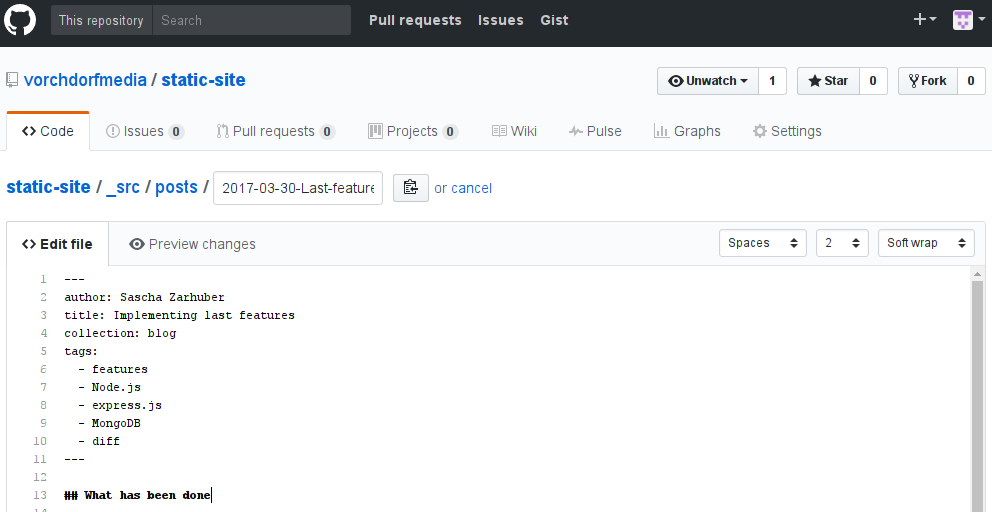
\includegraphics[width=0.9\textwidth]{github-page-editor.png}
    \caption{A Screenshot showing the \emph{In-Page Code Editor} of GitHub. An existing file is selected and ready to be edited. When finished, the user may commit the changes into the repository, so that other contributors also benefit from his/her adjustments.}
    \label{fig:github-page-editor}
\end{figure}
%

Especially for content authors without programming knowledge, the \emph{In-Page Code Editor} might be a very supportive tool, as it provides a clean and easy-to-use frontend for directly adding content to the repository (see Fig. \ref{fig:github-page-editor}). Additionally, the just edited file may not only be committed into the currently selected branch, but also in a newly created branch. Therefore, the source branch stays clean, whereas the edited file may get reviewed by an assigned supervisor, before being ready to get merged.\\
Furthermore, also developers might make use of this feature, especially when a small hotfix is to be made, where it would be too time-consuming to \emph{pull, commit} and \emph{push} from/to the repository \cite[405]{loeliger2012version}.

Pushing to a \emph{gh-pages} branch, or creating a \emph{<username>.github.io} repository, enables the use of GitHub's built-in website hosting service. From there, either a Jekyll project is freshly built, or already compiled static HTML are automatically published to the web -- additionally, custom domains may be used when adding a \texttt{CNAME} file \cite[p. 171f]{dhillon2016}.

\subsection{REST API}
Another significant advantage is the access of GitHub's REST API. Currently existing in its third major release, it almost offers every feature also available graphically in its web interface, as an equivalent JavaScript Object Notation (\emph{JSON}) upon programmatical request. Some services even feature more advanced data through the API than through the UI \cite[410]{loeliger2012version}.

When having the need of including data from a GitHub account into a third party service, a single authenticated HTTP request does the trick. Due to many available endpoints, a developer may quickly find the type information he/she needs to further process data directly from a repository. As an example, a complete listing of a repository's file tree is also possible, without needing to download and unpack an archive file. For one thing, this saves quite some time, for another thing, the requested data is already processed and presented, so that not only file paths are unveiled, but also their direct links and data types.

Furthermore, the API not only offers access to informational data about a given repository, instead, its manipulation through creating commits or uploading a file may also happen. To sum this up, very well documented examples are available on the API page on GitHub, where developers catch a good glimpse, of what is possible overall\footnote{\url{https://developer.github.com/v3/} -- API v3 documentation on GitHub.} \cite[401]{loeliger2012version}.


\section{Diff}
\label{sec:diff}

``\emph{diff} reports file differences between two files, expressed as a minimal list of line changes (\ldots)'' \cite[1]{Hunt1976}. Existing more than 40 years now, it has been an essential tool for file comparison throughout the history of computing -- furthermore, it is also a core component of Git, which contains its own version called \emph{git diff} \cite[108]{loeliger2012version}.

\subsection{History}
\label{sec:diff-history}
Initially published by \emph{James W. Hunt} and \emph{Malcolm D. McIlroy} in July 1976 when working at \emph{Bell Labs}, the algorithm was later used in \emph{UNIX} as application called diff. \emph{Paul Eggert} and \emph{Richard Stallman} (among others) also wrote the diff application as part of their \emph{GNU diffutils}\footnote{\url{http://manpages.ubuntu.com/manpages/zesty/en/man1/diff.1.html} -- Manpage for GNU diff.}, which is nowadays mainly distributed in Linux derivatives, MacOS, as well as part of Git. They used an improved algorithm published by \emph{Webb Miller} and \emph{Eugene W. Myers} in 1985 \cite[3]{mackenzie2003comparing}, who proved, that the original ``Hunt-McIlroy algorithm'' is inefficient on certain special cases. As a test case, they used a file containing 1000 blank lines, and a second file, consisting of the initial file, but containing a single non-blank file on both ends. As a fact, using other experiments performed on typical files, Miller's and Myers' algorithm ran roughly four times faster \cite[p. 1034f]{miller1985file}.

\subsection{Technology}
\label{sec:diff-technology}

\begin{lstlisting}[label={list:diff-normalformat}, caption=sample.diff]
0a1
> w
3,4c4,6
< c
< d
---
> x
> y
> z
6,7d7
< f
< g
\end{lstlisting}

diff's core task is finding the ``shortest sequence of insertions and deletions that will convert the first string to the second'' \cite[1025]{miller1985file} together with finding the longest common subsequence occurring in both files \cite[2]{Hunt1976}. Combined with the mathematical algorithm, it should provide an easily understandable format for humans, consisting of line numbers joined with \emph{a, c} or \emph{d} (append, change, delete), as well as \emph{<} and \emph{>} line prefixes, showing the affiliation either to the initial or compared file. This is called the ``Normal Format'' \cite[12]{mackenzie2003comparing}. Listing \ref{list:diff-normalformat} shows a sample output, comparing the strings \texttt{a b c d e f g} and \texttt{w a b x y z e} (one line per letter)\cite[p. 1f]{Hunt1976}.


% TODO: Ugly, remove if not necessary anymore, cares for vertical spaces above subsections
\vspace{20pt}
\subsubsection{The Unified Format}

To provide a more readable user experience, GNU diff contains an improved format, called Unified Format, removing redundancy by using a more compact syntax. It can be selected as output format by executing diff together with a \texttt{-u} flag \cite[16]{mackenzie2003comparing}, whereas git diff uses this as standard format to show changes within the current working tree \cite{GitDiff}.


\begin{lstlisting}[label={list:diff-unifiedformat}, caption=unified\_format.diff]
--- oldfile	2017-04-13 09:42:47.474769553 +0200
+++ newfile	2017-04-13 09:43:13.898566935 +0200
@@ -1,7 +1,7 @@
+w
 a
 b
-c
-d
+x
+y
+z
 e
-f
-g
\end{lstlisting}

As an example, listing \ref{list:diff-unifiedformat} shows the same diff output as listing \ref{list:diff-normalformat}, only as Unified Format using the following components:

\begin{description}
  \item[\texttt{------ \{filename\} \{timestamp\}}] -- indicates the initial file together with the timestamp it was created,
  \item[\texttt{+++ \{filename\} \{timestamp\}}] -- same as above, but for the compared file
  \item[\texttt{@@ -\{intial line range\} +\{compared line range\} @@}] -- \texttt{-1,7} indicates the following 7 lines, starting from the first line of the initial file
  \item[\texttt{+}] -- marks a line as added in compared file
  \item[\texttt{-}] -- marks a line as deleted in compared file
\end{description}

To make the above explanation a little bit more clear, an additional example with a text speaking for itself is added below:

\lstinputlisting[caption={file.diff}, label={list:diff-explanation}]{chapters/03-technical-foundations/_support/file.txt}

It can be clearly seen, that line 3 shows a growth of \emph{newfile} by two lines: -1,8 vs. +1,10. Having also a color-coded representation, it would boost the readability of such diff outputs once again.


% TODO: Ugly, remove if not necessary anymore, cares for vertical spaces above subsections
%\vspace{20pt}
\subsubsection{Usage with Git}
As already stated, diff is one of the core components of Git. Not only does it support determining changes in the source code between a snapshot and another, it may also reveal merge conflicts, if segments are mutually exclusive and therefore preventing a flawless propagation of development. Thus, a varying development history of different origins (e.g. branches) not compatible to each other might be indicated. Furthermore, a conflict may also happen, if a developer forgot to \emph{pull} the latest changes before committing his/her current development progress. These conflicts may only be handled through human guidance \cite[124]{loeliger2012version}.

\begin{lstlisting}[label={list:diff-conflict}, caption={A snippet of a file called ``manual.txt'', which is affected by a conflict. Content between \texttt{HEAD} and \texttt{=======} contains the local version, content below contains the foreign conflicting version.}]
<<<<<<< HEAD:manual.txt
I (the developer) am right!
=======
The branch_name is right!
>>>>>>> branch_name:manual.txt
\end{lstlisting}

A conflict presents itself primarily through a message similar to:\\
\texttt{CONFLICT (content): Merge conflict in file\\
Automatic merge failed; fix conflicts and then commit the result.}\\
If anything like the above happens, the affected files by the conflict also contain a structure like shown in listing \ref{list:diff-conflict}. A conflict can then be resolved by removing its markers and picking the appropriate resolution of either side of the \texttt{=======} delimiter \cite{GitConflicts}, as well as mixing them to the developers needs \cite[126]{loeliger2012version}. A single file may also contain multiple conflicts.

\subsubsection{Usage with GitHub}
Especially when interacting with GitHub's REST API, it is very easy to generate and import file diffs of a given repository. Whether two branches or two commits using their \emph{SHA} values are compared, a single HTTP request suffices for programmatically retrieving data, which is normally only accessible using a terminal emulator.

Depending on the requested \emph{media type} in the appropriate HTTP header field, either a full-featured diff, patch or JSON containing per-file patches is emitted by the API. If the latter was used, the underlying diff is translated into a JSON object, containing information like the number of additions, deletions and changes, as well as the mentioned \emph{patch} for each file.

As a consequence, a repository does not necessarily have to be \emph{cloned}, as it may be patched constantly using the API to keep it up to date -- using this method, patch is even able to create and delete files, if necessary \cite[57]{mackenzie2003comparing}. The only prerequisite is to keep track of the single commit hashes the patches are applied from.

